% template adapted from https://github.com/jgm/pandoc-templates/blob/master/default.latex
%%%%%%%%%%%%%%%%%%%%%%%%%%%%%%%%%%%%%%%%%%%%%%%%%%%%%%%%%%%%%%%%%%%%%%%%%%%%%%%%%%%%%%%%%

% Options for packages loaded elsewhere
\PassOptionsToPackage{unicode=true}{hyperref}
\PassOptionsToPackage{hyphens}{url}
  \PassOptionsToPackage{dvipsnames,svgnames*,x11names*}{xcolor}


\documentclass[
  11pt,
  french,
  a4paper,
  extrafontsizes,onecolumn,openright
  ]{memoir}

% Font family: lmodern by default
  \usepackage{lmodern}

% Double (or whatever) spacing

\usepackage{amssymb, amsmath}
\usepackage{ifxetex,ifluatex}

% mathspec: arbitrary math fonts
  \usepackage{unicode-math}
\defaultfontfeatures{Ligatures=TeX,Scale=MatchLowercase}

% More font families
% Main font
% Specific sanserif font
% Specific monotype font
% Specific math font
% Chinese, Japanese, Corean fonts

% Use upquote if available, for straight quotes in verbatim environments
\IfFileExists{upquote.sty}{\usepackage{upquote}}{}
% Use microtype if available
\IfFileExists{microtype.sty}{%
\usepackage[]{microtype}
\UseMicrotypeSet[protrusion]{basicmath} % disable protrusion for tt fonts
}{}

% Verbatim in note

\usepackage{xcolor}


% Geometry package

% Listings package


\usepackage{color}
\usepackage{fancyvrb}
\newcommand{\VerbBar}{|}
\newcommand{\VERB}{\Verb[commandchars=\\\{\}]}
\DefineVerbatimEnvironment{Highlighting}{Verbatim}{commandchars=\\\{\}}
% Add ',fontsize=\small' for more characters per line
\usepackage{framed}
\definecolor{shadecolor}{RGB}{248,248,248}
\newenvironment{Shaded}{\begin{snugshade}}{\end{snugshade}}
\newcommand{\AlertTok}[1]{\textcolor[rgb]{0.94,0.16,0.16}{#1}}
\newcommand{\AnnotationTok}[1]{\textcolor[rgb]{0.56,0.35,0.01}{\textbf{\textit{#1}}}}
\newcommand{\AttributeTok}[1]{\textcolor[rgb]{0.77,0.63,0.00}{#1}}
\newcommand{\BaseNTok}[1]{\textcolor[rgb]{0.00,0.00,0.81}{#1}}
\newcommand{\BuiltInTok}[1]{#1}
\newcommand{\CharTok}[1]{\textcolor[rgb]{0.31,0.60,0.02}{#1}}
\newcommand{\CommentTok}[1]{\textcolor[rgb]{0.56,0.35,0.01}{\textit{#1}}}
\newcommand{\CommentVarTok}[1]{\textcolor[rgb]{0.56,0.35,0.01}{\textbf{\textit{#1}}}}
\newcommand{\ConstantTok}[1]{\textcolor[rgb]{0.00,0.00,0.00}{#1}}
\newcommand{\ControlFlowTok}[1]{\textcolor[rgb]{0.13,0.29,0.53}{\textbf{#1}}}
\newcommand{\DataTypeTok}[1]{\textcolor[rgb]{0.13,0.29,0.53}{#1}}
\newcommand{\DecValTok}[1]{\textcolor[rgb]{0.00,0.00,0.81}{#1}}
\newcommand{\DocumentationTok}[1]{\textcolor[rgb]{0.56,0.35,0.01}{\textbf{\textit{#1}}}}
\newcommand{\ErrorTok}[1]{\textcolor[rgb]{0.64,0.00,0.00}{\textbf{#1}}}
\newcommand{\ExtensionTok}[1]{#1}
\newcommand{\FloatTok}[1]{\textcolor[rgb]{0.00,0.00,0.81}{#1}}
\newcommand{\FunctionTok}[1]{\textcolor[rgb]{0.00,0.00,0.00}{#1}}
\newcommand{\ImportTok}[1]{#1}
\newcommand{\InformationTok}[1]{\textcolor[rgb]{0.56,0.35,0.01}{\textbf{\textit{#1}}}}
\newcommand{\KeywordTok}[1]{\textcolor[rgb]{0.13,0.29,0.53}{\textbf{#1}}}
\newcommand{\NormalTok}[1]{#1}
\newcommand{\OperatorTok}[1]{\textcolor[rgb]{0.81,0.36,0.00}{\textbf{#1}}}
\newcommand{\OtherTok}[1]{\textcolor[rgb]{0.56,0.35,0.01}{#1}}
\newcommand{\PreprocessorTok}[1]{\textcolor[rgb]{0.56,0.35,0.01}{\textit{#1}}}
\newcommand{\RegionMarkerTok}[1]{#1}
\newcommand{\SpecialCharTok}[1]{\textcolor[rgb]{0.00,0.00,0.00}{#1}}
\newcommand{\SpecialStringTok}[1]{\textcolor[rgb]{0.31,0.60,0.02}{#1}}
\newcommand{\StringTok}[1]{\textcolor[rgb]{0.31,0.60,0.02}{#1}}
\newcommand{\VariableTok}[1]{\textcolor[rgb]{0.00,0.00,0.00}{#1}}
\newcommand{\VerbatimStringTok}[1]{\textcolor[rgb]{0.31,0.60,0.02}{#1}}
\newcommand{\WarningTok}[1]{\textcolor[rgb]{0.56,0.35,0.01}{\textbf{\textit{#1}}}}

% Tables
  \usepackage{longtable,booktabs,tabu}
  % Fix footnotes in tables (requires footnote package)
  \IfFileExists{footnote.sty}{\usepackage{footnote}\makesavenoteenv{longtable}}{}

% Graphics
  \usepackage{graphicx,grffile}
  \graphicspath{{images/}}
  \makeatletter
  \def\maxwidth{\ifdim\Gin@nat@width>\linewidth\linewidth\else\Gin@nat@width\fi}
  \def\maxheight{\ifdim\Gin@nat@height>\textheight\textheight\else\Gin@nat@height\fi}
  \makeatother
  % Scale images if necessary, so that they will not overflow the page
  % margins by default, and it is still possible to overwrite the defaults
  % using explicit options in \includegraphics[width, height, ...]{}
  \setkeys{Gin}{width=\maxwidth,height=\maxheight,keepaspectratio}



\setlength{\emergencystretch}{3em}  % prevent overfull lines
\providecommand{\tightlist}{%
  \setlength{\itemsep}{0pt}\setlength{\parskip}{0pt}}

  \setcounter{secnumdepth}{5}

% set default figure placement to htbp
\makeatletter
\def\fps@figure{htbp}
\makeatother

% Include headers (preamble.tex) here
%%% Complete the preamble of the LaTeX template
%%%------------------------------------------------------------------------------

%%% PACKAGES
\usepackage{lipsum} % Dummy text.

% Bug de bookdown: ne traite plus la déclaration "otherlangs" dans le préambule
% Pour charger les langues, écriture ici en dur du produit de bookdown
% Corrigé le 22/11/2019. A retester régulièrement: supprimer ces lignes si la compilation fonctionne sans elles.
\usepackage{polyglossia}
  \setmainlanguage[variant=american]{english}
  \setotherlanguage[]{french}

% Environnement "Essentiel" en début de chapitre
\usepackage[tikz]{bclogo}
\newenvironment{Essentiel}
  {\begin{bclogo}[logo=\bctrombone, noborder=true, couleur=lightgray!50]{L'essentiel}\parindent0pt}
  {\end{bclogo}}
% Utilisation :
%
%```{block, type='Essentiel'}
% Texte à mettre en valeur
% ```

\usepackage{enumitem}

  % load polyglossia as late as possible as it *could* call bidi if RTL lang (e.g. Hebrew or Arabic)
  \usepackage{polyglossia}
  \setmainlanguage[]{french}




\usepackage[style=authoryear-ibid,backend=biber,citestyle=verbose-inote,pageref=true,isbn=false,backref=true,giveninits=true,uniquename=init,maxcitenames=2,maxbibnames=150,sorting=nyt,sortcites=false]{biblatex}
\addbibresource{MyBook.bib}
\addbibresource{packages.bib}

% cslreferences environment required by pandoc > 2.7


% Specific commands for EcoFoG style. Must come after biblatex.
\usepackage{latex/BookTemplate}

% Hyperref comes last
\usepackage{hyperref}
\hypersetup{
            pdftitle={Ouvrage Bookdown},
            pdfauthor={Prénom NomAuteur},
            pdfkeywords={Keyword in English, As a list},
            colorlinks=true,
            linkcolor=Maroon,
            citecolor=Blue,
            urlcolor=Blue,
            breaklinks=true}

% Don't use monospace font for urls
\urlstyle{same}


% Title, author, etc. from YAML to LaTeX
%%%%%%%%%%%%%%%%%%%%%%%%%%%%%%%%%%%%%%%%%%%%%%%%%%%%%%%%%%

\title{Ouvrage Bookdown}


\author{Prénom NomAuteur}


\date{2020-04-25}


% Main title page with filigrane
%%%%%%%%%%%%%%%%%%%%%%%%%%%%%%%%%%%%%%%%%%%%%%%%%%%%%%%%%%

\newcommand{\MainTitlePage}[1][]{
	\SmallMargins % Margins
	\pagestyle{empty} % No header/footer
	~\\ % Print a character or the page will not exist
	\begin{textblock}{2}(30,10)
		\rule{1pt}{\paperheight-20mm}
	\end{textblock}
	\begin{textblock}{140}(50, 45)
		\flushright
		\begin{Spacing}{3}
			{\fontfamily{qtm}\selectfont\fontsize{45}{45}\selectfont \textsc{\thetitle}}
		\end{Spacing}
	\end{textblock}
	\begin{textblock}{140}(50, 125)
		\flushright
		{\fontfamily{qtm}\Large \theauthor}
	\end{textblock}
	\begin{textblock}{120}[1, 1](225, 297)
		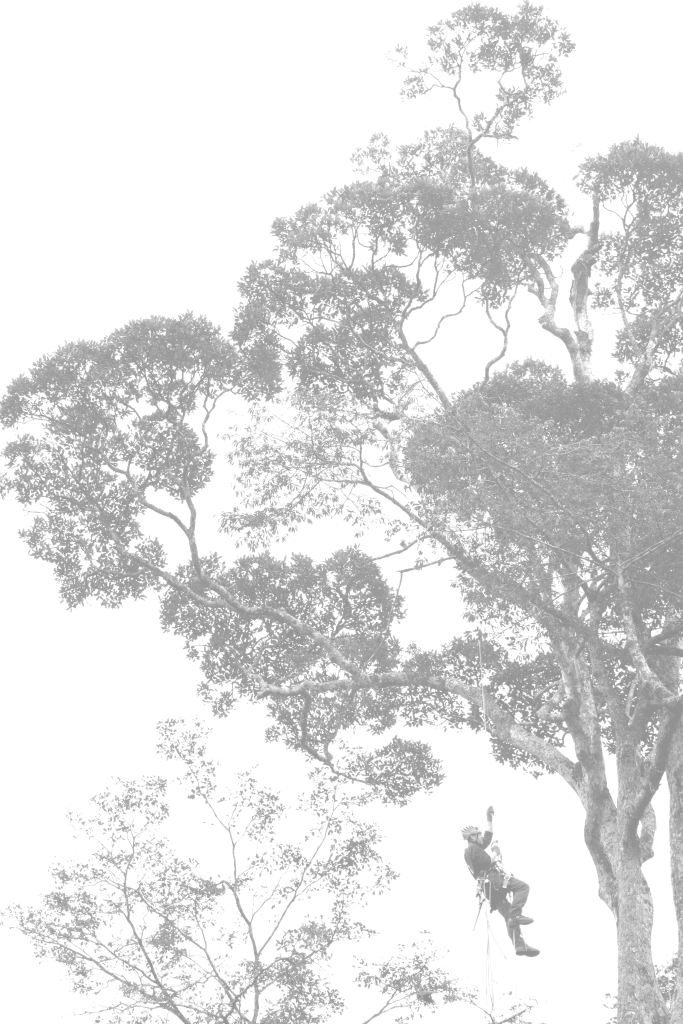
\includegraphics[width=10cm]{Filigrane}
	 \end{textblock}
	\begin{textblock}{140}[0, 1](50, 262)
		\normalfont	Version: \thedate
	\end{textblock}
	\newpage
	~\\ % Print a character or the page will not exist
	\begin{textblock}{140}(40, 40)
		#1
	\end{textblock}
	\begin{textblock}{140}[0,1](40, 270)
		\centering
    
\includegraphics[width=5cm]{Logo-Lab}\\ \bigskip
		UMR \'Ecologie des forêts de Guyane\\
		\url{http://www.ecofog.gf}\\[3\baselineskip]
		Les opinions émises par les auteurs sont personnelles et n’engagent ni l’UMR EcoFoG ni ses tutelles.

    \tiny{Photographie en couverture: Hadrien Lalagüe}
	\end{textblock}
	\newpage
}

% PhD / HDR Thesis
%%%%%%%%%%%%%%%%%%%%%%%%%%%%%%%%%%%%%%%%%%%%%%%%%%%%%%%%%%

\usepackage[DocType=PhD, ED=UG, Ets=UG, DIS=ST]{latex/pdgUniv}

\specialty{Écologie}
\defencedate{1er janvier 2018}
\lab{Écologie des Forêts de Guyane}
% ==================
% Setup people like your boss, the jury team and the referees
% - First you need to define how number they will be in each category
%   It is done with the commands \nboss{n}, \nreferee{n} and \njudge{n}.
%   You can define more people in each category than the number given
%   but only the first "\npeople" will be print.
% - Then use the command \makesomeone{<category>}{<number>}{<name>}{<status>}{<other>}
%   where:
%     <category> should be select in ['boss', 'referee', 'judge']
%     <number>   is the rank for printing the person.
%                Only number <= "\npeople" will be printed
%     <name>     First name and las name of the people
%     <status>   Is (s)he a "charg\'e de recher" ou un "professeur d'universit\'e"...
%     <other>    What ever string you want to add (laboratory, jury member place...).
\njudge{7}
\makesomeone{judge}{1}{Prénom NomJury1}{Professeur d'Université}{Membre du Jury}
\makesomeone{judge}{2}{Prénom NomJury2}{Professeur d'Université}{Membre du Jury}
\makesomeone{judge}{3}{Prénom NomJury3}{Professeur d'Université}{Membre du Jury}
\makesomeone{judge}{4}{Prénom NomJury4}{Professeur d'Université}{Membre du Jury}
\makesomeone{judge}{5}{Prénom NomJury5}{Professeur d'Université}{Membre du Jury}
\makesomeone{judge}{6}{Prénom NomJury6}{Professeur d'Université}{Membre du Jury}
\makesomeone{judge}{7}{Prénom NomJury7}{Professeur d'Université}{Membre du Jury}



% End of preamble
%%%%%%%%%%%%%%%%%%%%%%%%%%%%%%%%%%%%%%%%%%%%%%%%%%%%%%%%%%


\begin{document}
\frontmatter

% Title page
%%%%%%%%%%%%%%%%%%%%%%%%%%%%%%%%%%%%%%%%%%%%%%%%%%%%%%%%%%

\MainTitlePage[Texte optionnel ajouté en haut de la page au verso du titre du document.

Exemple:

Ce document est réalisé de façon dynamique et reproductible grâce à:

\begin{itemize}
  \item \LaTeX, dans sa distribution Miktex (\url{http://miktex.org/}) et la classe memoir (\url{http://www.ctan.org/pkg/memoir}).
  \item R (\url{http://www.r-project.org/}) et RStudio (\url{http://www.rstudio.com/})
  \item bookdown (\url{http://bookdown.org/})
\end{itemize}]

\makeflyleaf
\newpage
~
\newpage




% Before Body
%%%%%%%%%%%%%%%%%%%%%%%%%%%%%%%%%%%%%%%%%%%%%%%%%%%%%%%%%%




% Contents
%%%%%%%%%%%%%%%%%%%%%%%%%%%%%%%%%%%%%%%%%%%%%%%%%%%%%%%%%%

\LargeMargins
{
\hypersetup{linkcolor=}
\setcounter{tocdepth}{3}
\tableofcontents
}


% Body
%%%%%%%%%%%%%%%%%%%%%%%%%%%%%%%%%%%%%%%%%%%%%%%%%%%%%%%%%%

\LargeMargins
\hypertarget{principes}{%
\chapter*{Principes}\label{principes}}
\addcontentsline{toc}{chapter}{Principes}

Ce document permet de créer un livre au format PDF (et au format ePub) en même temps qu'une version HTML à publier sur le web.
La syntaxe est celle de \textbf{Markdown} avec quelques extensions.

Le package \textbf{bookdown} doit être installé à partir de CRAN ou GitHub:

\scriptsize

\begin{Shaded}
\begin{Highlighting}[]
\KeywordTok{install.packages}\NormalTok{(}\StringTok{"bookdown"}\NormalTok{)}
\CommentTok{# or the development version}
\CommentTok{# devtools::install_github('rstudio/bookdown')}
\end{Highlighting}
\end{Shaded}

\normalsize

Le livre est organisé en chapitres.
Chaque chapitre est un fichier Rmd, dont le nom commence normalement par son numéro (ex.: 01-intro.Rmd).
Tous les fichiers Rmd présents dans le dossier du projet sont en réalité traités comme des chapitres, triés par ordre de nom de fichier.
Le fichier index.Rmd est particulier: il contient l'entête du document et le premier chapitre.

Ce premier chapitre est placé dans l'avant-propos de l'ouvrage imprimé: il ne doit pas être numéroté (d'où le code \texttt{\{-\}} à côté du titre) dans la version HTML. Il se termine obligatoirement par la commande LaTeX \texttt{\textbackslash{}mainmatter} qui marque le début du corps de l'ouvrage.

Les niveaux de plan commencent sont \texttt{\#} pour les chapitres (un seul par fichier), \texttt{\#\#} pour les sections, etc.

La compilation au format PDF est faite par XeLaTeX, qui doit être installé.

Pendant la rédaction, il est fortement conseillé de ne créer que le fichier HTML, ce qui est beaucoup plus rapide qu'une compilation LaTeX.
Chaque chapitre peut être visualisé très rapidement en cliquant sur le bouton \emph{Knit} au-dessus de la fenêtre de source.
Le livre entier est créé en cliquant sur le bouton \emph{Build Book} de la fenêtre \emph{Build} de RStudio.
La liste déroulante du bouton permet de créer tous les documents ou de se limiter à un format.

\mainmatter

\hypertarget{Demarrage}{%
\chapter{Démarrage}\label{Demarrage}}

\emph{RStudio} en version supérieure à 1 doit être utilisé.
Le package \textbf{bookdown} doit être installé.

Pour la création du fichier PDF, une installation de LaTeX est nécessaire.
Sous Windows, utiliser \href{https://miktex.org/download}{MikTex}.
Le téléchargement automatique des packages manquants (sous Windows: MiKTeX settings, \emph{Install missing packages=Yes}) est indispensable.

Les paramètres de base du projet doivent être saisis dans les fichiers suivants.

\hypertarget{index.rmd}{%
\section{index.Rmd}\label{index.rmd}}

Dans l'entête du fichier, saisir le titre de l'ouvrage et le nom du ou des auteurs

\begin{verbatim}
title: "Ouvrage Bookdown" 
author: "Prénom NomAuteur"
\end{verbatim}

Les options spécifiques à LaTeX sont:

\begin{itemize}
\item
  \emph{documentclass} la classe de document, obligatoirement \emph{memoir} pour ce modèle. Les options de la classe \emph{memoir} sont énumérer, à ne pas modifier normalement;
\item
  \emph{fontfamily}: la \href{https://en.wikibooks.org/wiki/LaTeX/Fonts\#Font_families}{police de caractère}, \emph{lmodern} par défaut;
\item
  \emph{linestretch}: l'interlignage, 1 par défaut;
\item
  \emph{papersize}: A4;
\item
  \emph{fontsize}: 11pt;
\item
  \emph{toc-depth}: nombre de niveaux dans la table des matières, 3 par défaut;
\item
  \emph{lang}: fr ou en-US ou en-GB, la langue principale;
\item
  \emph{otherlangs}: les autres langues utilisées dans le document, par défaut {[}en-US, en-GB, fr{]};
\item
  \emph{graphics}: yes obligatoirement pour utiliser le package \emph{graphics} nécessaire aux figures;
\item
  \emph{fig\_crop}: yes pour autoriser le rognage des marges excédentaires des figures;
\item
  La quatrième de couverture affichera le résumé en Français et en Anglais et les mots-clés associés si les instructions \emph{resume}, \emph{mots-cles}, \emph{abstract} et \emph{keywords} sont présentes;
\item
  \emph{fourthpagefontsize} donne la taille de la police de caractère de la quatrième de couverture, normalsize par défaut, à adapter selon la longueur des résumés. La commande doit être reconnue par LaTeX.
\end{itemize}

Les paramètres de la bibliographie sont:

\begin{itemize}
\item
  \emph{bibliography}: fichiers contenant les références, {[}MyBook.bib, packages.bib{]} par défaut. \emph{package.bib} est créé par le premier bout de code du document: il permet de citer les packages déclarés avec les identifiants de la forme \texttt{@R-package}. R lui-même est cité par \texttt{@R-base};
\item
  \emph{biblio-style}: le style bibliographique, authoryear-ibid par défaut;
\item
  \emph{cite-style}: le style des citations dans le document LaTeX, verbose-inote par défaut;
\item
  \emph{biblatexoptions} contient la liste des options de biblatex, utilisées pour la production du document PDF;
\item
  \emph{link-citations}: yes pour que les citations soient des liens hypertexte;
\item
  \emph{colorlinks}: yes pour que les liens hypertexte soient affichés en couleur.
\end{itemize}

La couverture sera:

\begin{itemize}
\item
  au format livre si l'instruction \emph{maintitlepage} est présente. Le contenu de \emph{epigraph} sera écrit en page 2;
\item
  au format thèse si l'instruction \emph{PhD-HDR} est présente. Préciser alors:

  \begin{itemize}
  \item
    DocType: type de document, thèse (PhD) ou HDR;
  \item
    ED: école doctorale (UG ou UA);
  \item
    Ets: étalissement délivrant le diplôme (UG, UA ou APT);
  \item
    DIS: discipline (ST, SAN, ALL, DSE, SHS pour Sciences et Technologies; Santé; Arts, Lettres, Langues; Droit, Sciences Économiques et Gestion; Sciences Humaines et Sociales);
  \item
    speciality: texte libre, par exemple Écologie, mais la spécialité doit être validée par l'Ecole doctorale;
  \item
    defence-date: date de soutenance, en toutes lettres;
  \item
    lab: nom de l'unité de recherche, par exemple Écologie des Forêts de Guyane;
  \item
    njudge: Nombre de membres du jury, à énumérer ensuite:
  \item
    jury1: (numéroter le jury)

    \begin{itemize}
    \item
      category: judge obligatoirement dans l'organisation actuelle;
    \item
      name: Prénom et Nom du membre du jury;
    \item
      status: Texte libre, par exemple Professeur d'Université;
    \item
      other: rôle dans le jury: Membre du Jury, Président, Raporteur\ldots{}
    \end{itemize}
  \end{itemize}
\end{itemize}

\hypertarget{bookdown.yml}{%
\section{\_bookdown.yml}\label{bookdown.yml}}

Saisir le nom du fichier Rmd qui sera le résultat de la fusion de tous les chapitres et choisir s'il doit être détruit après usage.
Les options par défaut conviendront à la plupart des usages.

\begin{verbatim}
book_filename: "_Book"
delete_merged_file: true
\end{verbatim}

Si le projet est hébergé sur GitHub, indiquer son adresse.
Sinon, supprimer la ligne.

\begin{verbatim}
repo: "https://github.com/EcoFoG/BookTemplate"
\end{verbatim}

Il est inutile de compléter les mots-clés selon la langue de l'ouvrage.
Les options \emph{language} sont prises en charge par ailleurs.

\begin{verbatim}
language:
  ui:
    chapter_name: "Chapitre "
\end{verbatim}

\hypertarget{output.yml}{%
\section{\_output.yml}\label{output.yml}}

Personnaliser la table des matières au format HTML.

\begin{verbatim}
config:
  toc:
    before: |
      <li><a href="./">Ouvrage Bookdown</a></li>
    after: |
      <li><a href="https://github.com/EcoFoG/ (...)
\end{verbatim}

\hypertarget{syntaxe}{%
\chapter{Syntaxe}\label{syntaxe}}

La syntaxe de \emph{R Mardown} étendue par \emph{Bookdown} est rappelée ici, en Anglais.

Les références bibliographiques \autocite{xie2015} sont supportées.

Le changement de langue est géré en LaTeX (ponctuation et césures différentes) mais pas en HTML.
La commande \texttt{\textbackslash{}selectlanguage\{english\}} est simplement ignorée en HTML.

\selectlanguage{english}

\hypertarget{section-in-english}{%
\section{Section in English}\label{section-in-english}}

You can label chapter and section titles using \texttt{\{\#label\}} after them, e.g., we can reference Chapter \ref{Demarrage}.

Figures and tables with captions will be placed in \texttt{figure} and \texttt{table} environments, respectively.

\scriptsize

\begin{Shaded}
\begin{Highlighting}[]
\KeywordTok{plot}\NormalTok{(pressure, }\DataTypeTok{type =} \StringTok{"b"}\NormalTok{, }\DataTypeTok{pch =} \DecValTok{19}\NormalTok{)}
\end{Highlighting}
\end{Shaded}

\begin{SCfigure}

{\centering 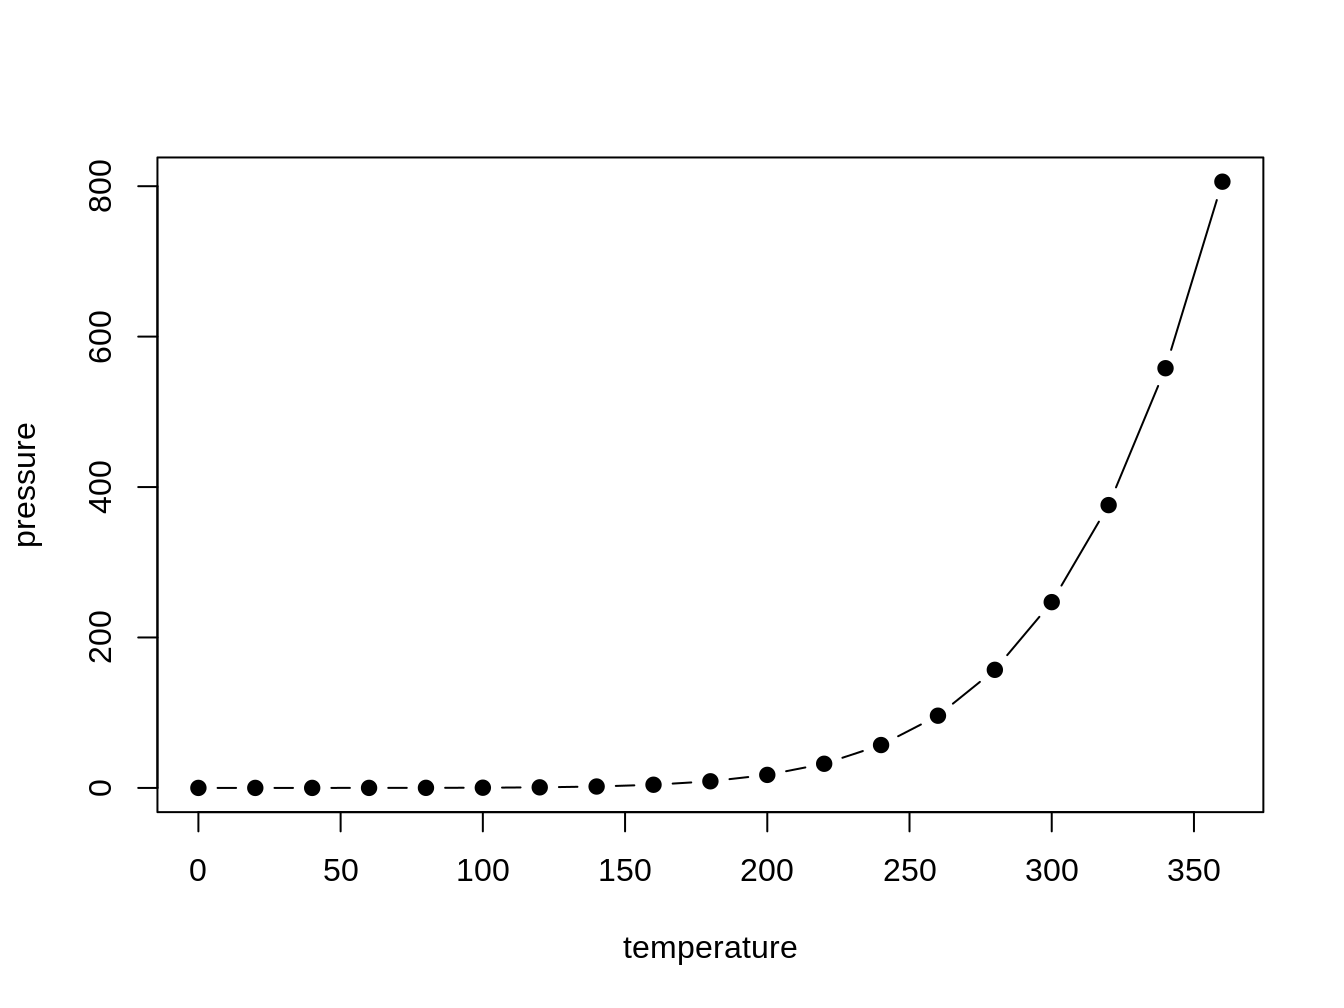
\includegraphics[width=0.8\linewidth]{MyBook_files/figure-latex/nice-fig-1} 

}

\caption{Here is a nice figure! It has a long, long, long, long, long, long, long, long, long, long, long, long, long, long, long, long, long, long, long, long, caption}\label{fig:nice-fig}
\end{SCfigure}

\normalsize

Reference a figure by its code chunk label with the \texttt{fig:} prefix, e.g., see Figure \ref{fig:nice-fig}. Similarly, you can reference tables generated from \texttt{knitr::kable()}, e.g., see Table \ref{tab:kable}.

\scriptsize

\begin{longtable}[t]{rrrrl}
\caption{\label{tab:kable}Tableau créé par R}\\
\toprule
Longueur sépales & Largeur & Longueur pétales & Largeur & Espèce\\
\midrule
5.1 & 3.5 & 1.4 & 0.2 & setosa\\
4.9 & 3.0 & 1.4 & 0.2 & setosa\\
4.7 & 3.2 & 1.3 & 0.2 & setosa\\
4.6 & 3.1 & 1.5 & 0.2 & setosa\\
5.0 & 3.6 & 1.4 & 0.2 & setosa\\
\addlinespace
5.4 & 3.9 & 1.7 & 0.4 & setosa\\
\bottomrule
\end{longtable}

\normalsize

\selectlanguage{french}

Remarque: si le tableau est mal formaté, supprimer le dossier \texttt{\_bookdown\_files} et recréer le livre.

La légende est précisée par l'argument \texttt{caption} et le référencement est possible parce que le tableau reçoit une étiquette dont le nom est \texttt{tab:} suivi du nom du bout de code (tableau \ref{tab:kable}).
Utiliser systématiquement l'argument \texttt{booktabs\ =\ TRUE} pour que l'épaisseur des lignes de séparation soit optimale en LaTeX.
L'option\break \texttt{bootstrap\_options\ =\ "striped"} fournit des tableaux plus lisibles en HTML.

En LaTeX, Les tableaux peuvent avoir la largeur de la colonne et éventuellement d'étendre sur plusieurs pages (\texttt{longtable\ =\ TRUE}).
L'option \texttt{longtable\ =\ FALSE} du modèle d'article pour afficher les tableaux en pleine largeur n'est pas disponible ici.

\hypertarget{documentation-pour-les-utilisateurs}{%
\section{Documentation pour les utilisateurs}\label{documentation-pour-les-utilisateurs}}

\begin{itemize}
\item
  L'ouvrage \href{https://bookdown.org/yihui/bookdown/}{bookdown: Authoring Books and Technical Documents with R Markdown} de Yihui Xie, l'auteur de \textbf{bookdown} et de \textbf{knitr}. Toutes les précisions nécessaires à la rédaction (écriture d'équations, références croisées, etc.) y sont données;
\item
  L'\href{https://www.rstudio.com/wp-content/uploads/2015/02/rmarkdown-cheatsheet.pdf}{anti-sèche de R Markdown} pour la syntaxe.
\end{itemize}

\hypertarget{documentation-pour-les-duxe9veloppeurs}{%
\section{Documentation pour les développeurs}\label{documentation-pour-les-duxe9veloppeurs}}

\begin{itemize}
\item
  La \href{http://rmarkdown.rstudio.com/pdf_document_format.html\#advanced_customization}{personnalisation du format du fichier LaTeX} produit.
\item
  Le \href{https://pandoc.org/MANUAL.html}{manuel de Pandoc} pour les options possibles dans l'entête YAML.
\end{itemize}


% Bibliography
%%%%%%%%%%%%%%%%%%%%%%%%%%%%%%%%%%%%%%%%%%%%%%%%%%%%%%%%%%

\backmatter
\SmallMargins

%
\printbibliography


% Tables (of tables, of figures)
%%%%%%%%%%%%%%%%%%%%%%%%%%%%%%%%%%%%%%%%%%%%%%%%%%%%%%%%%%




% After-body (LaTeX code inclusion)
%%%%%%%%%%%%%%%%%%%%%%%%%%%%%%%%%%%%%%%%%%%%%%%%%%%%%%%%%%



% Back cover
%%%%%%%%%%%%%%%%%%%%%%%%%%%%%%%%%%%%%%%%%%%%%%%%%%%%%%%%%%%

% Even page, small margins, no running head, no page number.
\evenpage
\SmallMargins
\thispagestyle{empty}

\begin{normalsize}

\begin{description}

\selectlanguage{french}
\item[Résumé:]
Résumé en Français, en quatrième de couverture.

Lorem ipsum dolor sit amet, consectetuer adipiscing elit. Maecenas porttitor congue massa. Fusce posuere, magna sed pulvinar ultricies, purus lectus malesuada libero, sit amet commodo magna eros quis urna.

Nunc viverra imperdiet enim. Fusce est. Vivamus a tellus.

\selectlanguage{french}
\item[Mots clés :]
Mot clé en Français, En liste.
~\\

\selectlanguage{english}
\item[Abstract:]
English abstract, on the last page.

Lorem ipsum dolor sit amet, consectetuer adipiscing elit. Maecenas porttitor congue massa. Fusce posuere, magna sed pulvinar ultricies, purus lectus malesuada libero, sit amet commodo magna eros quis urna.

Nunc viverra imperdiet enim. Fusce est. Vivamus a tellus.

\selectlanguage{english}
\item[Keywords:]
Keyword in English, As a list.

\end{description}

\end{normalsize}

\vspace*{\fill}
\centering
\includegraphics[width=.3\textwidth]{images/Logo-Lab}
\end{document}
